\subsection{Error evaluation with exact solution}
We study a numerical experiment with the exact solution of heat equation and evaluate the error convergence. Consider a square $[0,1]\times[0,1]$. Find $u(x,y,t)$ satisfied
\begin{equation}
\dfrac{\partial u}{\partial t} - \left(\dfrac{\partial^2 u}{\partial x^2} + \dfrac{\partial^2u}{\partial y^2}\right) = (1+2\pi^2)\sin(\pi x) \sin(\pi y)\exp(t),
\end{equation}
with the initial and boundary conditions
$$
u(x,y,0) = \sin(\pi x)\sin(\pi y)\exp(t) \quad \text{and} \quad u|_\Gamma = 0.
$$
The exact solution is
$$
u = \sin(\pi x) \sin(\pi y) \exp(t),
$$
%\begin{figure}[ht]	
%	\centering
%	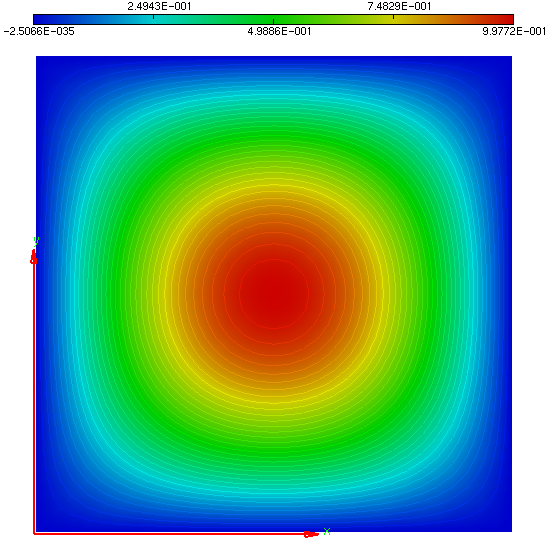
\includegraphics[width=0.8\linewidth]{figures/direct}
%	\caption{Exact solution of direct problem.} \label{fig:direct}
%\end{figure}
%The approximate solution at final time is illustrated in Figure \ref{fig:direct}.
Different cases of mesh size and time step length were studied to show the dependent of error on the mesh smoothness.
\begin{figure}[h!]
	\centering
	\begin{tabular}{c}
		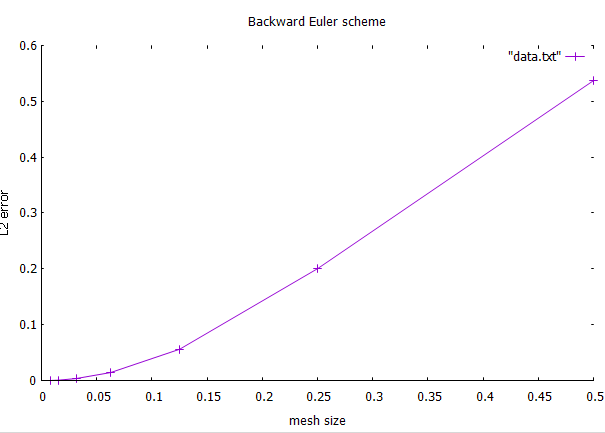
\includegraphics[width=.8\linewidth]{figures/BE} \\ 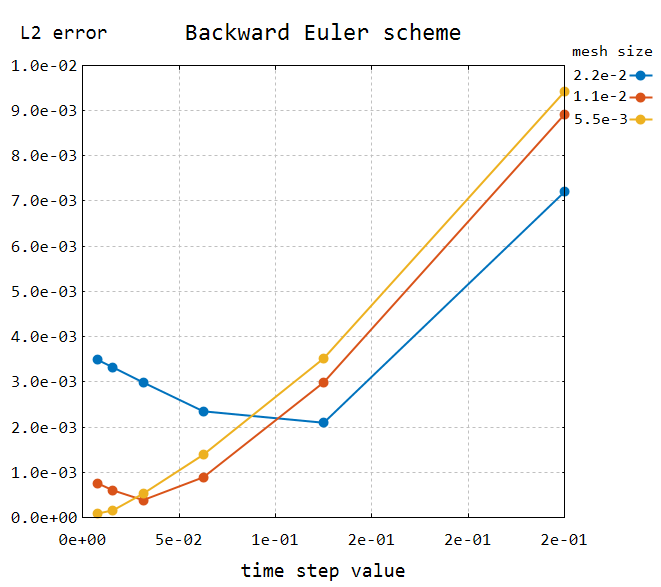
\includegraphics[width=.8\linewidth]{figures/BEt}
	\end{tabular}
	\caption{$L^2$ error convergence of Backward Euler scheme dependency on mesh size and time step.}
\end{figure}
\begin{figure}[h!]
	\centering
	\begin{tabular}{c}
		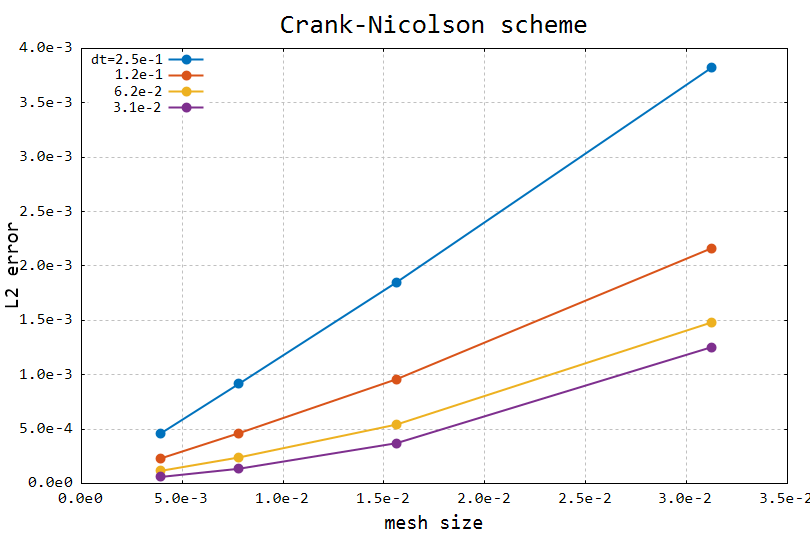
\includegraphics[width=.8\linewidth]{figures/CN} \\ 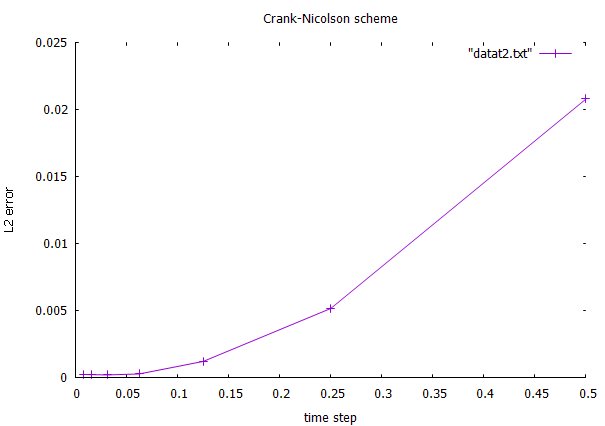
\includegraphics[width=.8\linewidth]{figures/CNt}
	\end{tabular}
	\caption{$L^2$ error convergence of Crank-Nicolson scheme dependency on mesh size and time step.}
\end{figure}

\subsection{A problem of thermal engineering}
We apply the numerical simulations of heat transfer into designing heat sink. Assuming a hot CPU inside a rectangular room fill with air. Let $u=u_{hot}$ inside CPU region and $u=u_{air}$ on air region, respectively $\Omega_{c}$ and $\Omega_{a}$, on the initial time. Our goal is to design a heat sink stick on the CPU to lower its temperature. \\
%\begin{figure}[ht]
%	\centering
%	\begin{tikzpicture}
%		\draw (-1,0) -- (2,0);
%		\draw (2,0) -- (2,3);
%		\draw (2,3) -- (-1,3);
%		\draw (-1,3) -- (-1,0);
%		\draw (0,0) -- (0,1);
%		\draw (0,1) -- (1,1);
%		\draw (1,1) -- (1,0);
%	\end{tikzpicture}
%\end{figure}
The heat sink region, denoted by $\Omega_{s}$, has thermal conductivity coefficient $\kappa_s$. Similarly, let $\kappa_a$ and $\kappa_c$ be respectively the thermal conductivity coefficients inside air and CPU region. Technically, $\kappa_a$ is small compare to $\kappa_c$ and $\kappa_s$ due to nature conduction of air. Furthermore, to provide cooling ability, $\kappa_s>\kappa_c$. The visualization using medit software.\\
\begin{figure}[h!]
	\centering
	\begin{tabular}{c}
		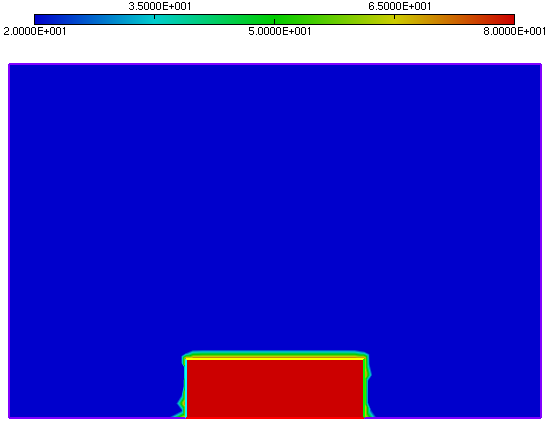
\includegraphics[width=.8\linewidth]{figures/begin}
	\end{tabular}
	\caption{Thermal distribution at initial state. $u|_{\Omega_{c}} = 80$, $u|_{\Omega_{a}\cup\Omega_{s}}=20$.}
\end{figure}
Set $T=1s$, $\kappa_a=0.01$, $\kappa_c=1$, $\kappa_s=100$. The temperature distribution at final time $T$ of different heat sink shapes are shown below.\\
\begin{figure}[h!]
	\centering
	\begin{tabular}{c}
		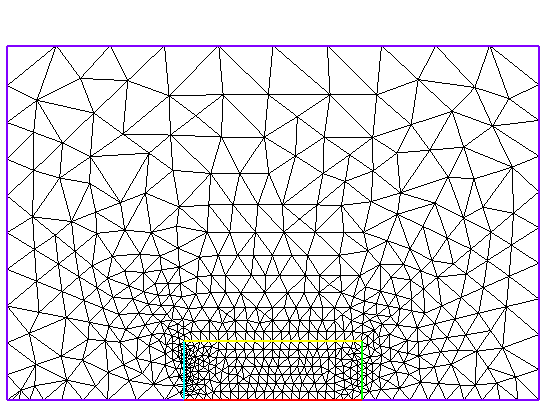
\includegraphics[width=.8\linewidth]{figures/nosinkc} \\ 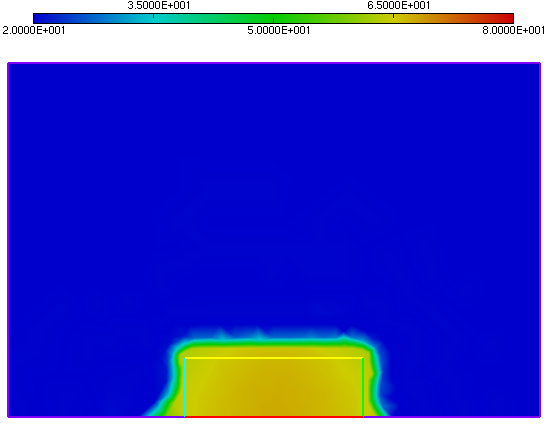
\includegraphics[width=.8\linewidth]{figures/nosinkb}
	\end{tabular}
	\caption{Thermal conduction with no heat sink. $u_{min}=63.1$, $u_{max}=67.3$.}
\end{figure}
\begin{figure}[h!]
	\centering
	\begin{tabular}{c}
		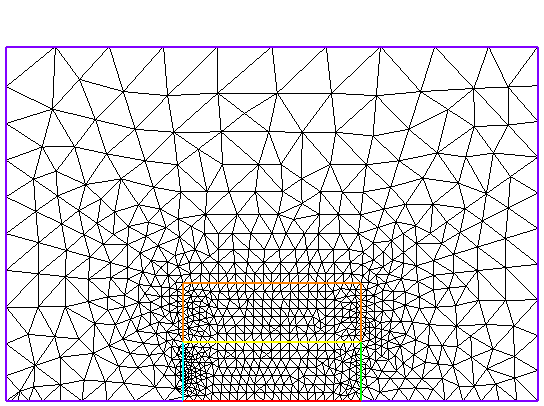
\includegraphics[width=.8\linewidth]{figures/recsinkc} \\ 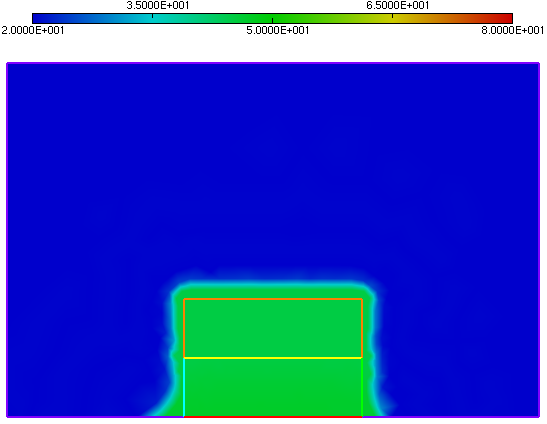
\includegraphics[width=.8\linewidth]{figures/recsinkb}
	\end{tabular}
	\caption{Thermal conduction with rectangular shape heat sink. $u_{min}=44.8$, $u_{max}=46.9$.}
\end{figure}
\begin{figure}[h!]
	\centering
	\begin{tabular}{c}
		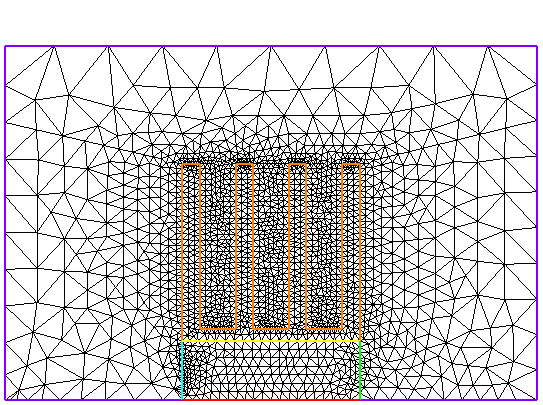
\includegraphics[width=.8\linewidth]{figures/finsinkc} \\ 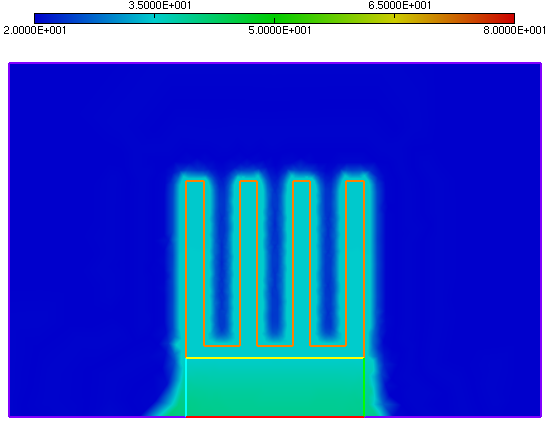
\includegraphics[width=.8\linewidth]{figures/finsinkb}
	\end{tabular}
	\caption{Thermal conduction with fin shape heat sink. $u_{min}=34.9$, $u_{max}=40.1$.}
\end{figure}
%\subsection{Numerical experiment of an optimal control problem}
%FreeFem++ provide an efficient tool to handle optimal control problem for partial differential equations by using the C++ optimization module IPOPT. To be more accurate, the module support multiple languages in solving optimization problems. The application of IPOPT for solving inverse heat problem is shown below.\\
%To use the IPOPT module we have to add command
%\begin{verbatim}
%load "ff-Ipopt"
%\end{verbatim}
%We need to find the expression of objective function $J$ and its gradient $\nabla J$ respective with the input control function $f$. The optimal $f$ is achieved via IPOPT loop using a conjugate gradient method solver such as Newton-Raphson method.
%\begin{verbatim}
%func real J(real[int] f) {
%Vh3 f3; f3[] = f;
%Vh3 u; u[] = StateProblem(f); 
%Vh3 del; del[] = u[] - w[];
%return 0.5 * int3d(Th3)(del * del) + 0.5 * gamma * int3d(Th3)(f3 * f3);
%}
%\end{verbatim}
%\begin{verbatim}
%func real[int] GradJ(real[int] f) {
%Vh3 p; p[] = AdjointProblem(StateProblem(f));
%Vh3 pq = p * q;
%real[int] res = pq[] + gamma * f;
%return res;
%}
%\end{verbatim}
%Execute the optimization with command
%\begin{verbatim}
%IPOPT(J, GradJ, fh[]);
%\end{verbatim}
%This is an illustrating of the expected control $f$ and its approximation using IPOPT. 

